掌握数据结构对开发者来说必不可少,大多数时候存储数据的方式决定了应用程序的效率。以电子邮件客户端为例,你可以设计一个电子邮件客户端,显示最近10封电子邮件,用户在使用你的应用两年内会收到数十万封电子邮件。当用户需要搜索电子邮件时,数据结构就会发挥重要作用。你储存成千上万封电子邮件的方式,排序和搜索它们的方法(算法)则非常重要。 \par
开发者在项目中努力寻找日常问题的最佳解决方案,使用经过验证的数据结构和算法可以极大地改善工作效率。好的程序最重要的特点是速度,我们可以通过设计新的算法,或使用现有的算法来得到良好的运行速度。 \par
最后,C++20引入了元类型的概念——描述其他类型的类型,这个强大特性使数据架构更加完整。 \par
C++标准模板库(STL)中包含了大量的数据结构和算法。我们将探索利用STL容器来使用数据结构有效地组织数据的方法,然后将深入研究STL提供的算法实现。理解和使用STL容器中的概念至关重要,因为C++20通过引入迭代器概念,对迭代器进行了重大改进。 \par
本章中,我们将了解以下内容: \par

\begin{itemize}
	\item 数据结构
	\item STL容器
	\item 概念和迭代器
	\item 主流算法
	\item 探索树和图
\end{itemize}

\noindent\textbf{}\ \par
\textbf{编译器要求} \ \par
g++编译器需要添加编译选项 \texttt{-std=c++2a} 来编译本章的代码。可以从这里获取本章的源码文件:https:/​/github.​com/PacktPublishing/Expert-CPP \par

\noindent\textbf{}\ \par
\textbf{数据结构} \ \par

\begin{center}
	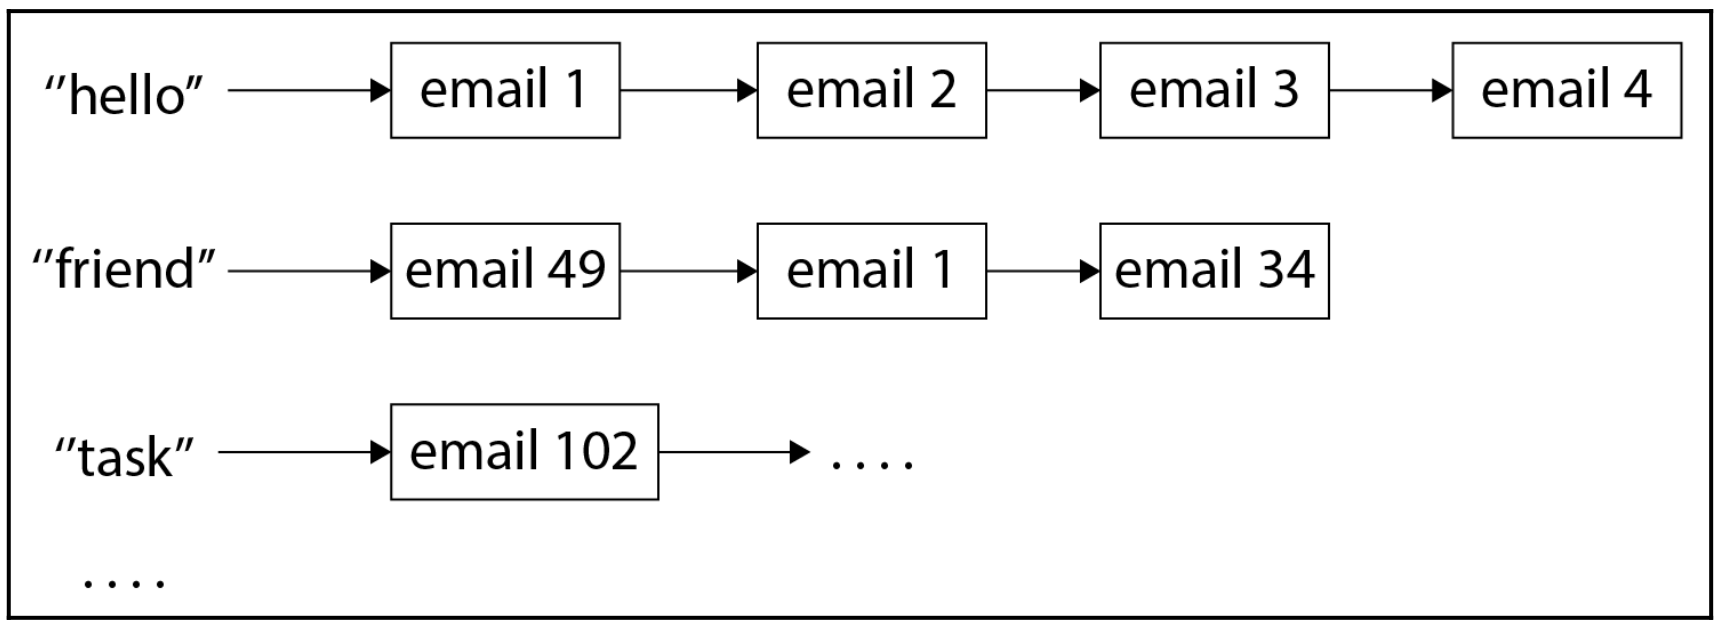
\includegraphics[width=0.6\textwidth]{content/Section-2/Chapter-6/1}
\end{center}

\noindent\textbf{}\ \par
\textbf{连续的数据结构} \ \par

\noindent\textbf{}\ \par
\textbf{节点式数据结构} \ \par

\noindent\textbf{}\ \par
\textbf{容器的内存} \ \par

\noindent\textbf{}\ \par
\textbf{STL容器} \ \par

\noindent\textbf{}\ \par
\textbf{使用std::vector和std::list} \ \par

\noindent\textbf{}\ \par
\textbf{使用容器适配器} \ \par

\noindent\textbf{}\ \par
\textbf{迭代容器} \ \par

\noindent\textbf{}\ \par
\textbf{概念和迭代器} \ \par

\noindent\textbf{}\ \par
\textbf{理解概念} \ \par

\noindent\textbf{}\ \par
\textbf{在C++20中使用迭代器} \ \par

\noindent\textbf{}\ \par
\textbf{主流算法} \ \par

\noindent\textbf{}\ \par
\textbf{搜索} \ \par

\noindent\textbf{}\ \par
\textbf{二分搜索} \ \par

\noindent\textbf{}\ \par
\textbf{排序} \ \par

\noindent\textbf{}\ \par
\textbf{搜索树和图} \ \par

\noindent\textbf{}\ \par
\textbf{哈希表} \ \par

\noindent\textbf{}\ \par
\textbf{图} \ \par

\noindent\textbf{}\ \par
\textbf{字符串} \ \par

\noindent\textbf{}\ \par
\textbf{总结} \ \par

\noindent\textbf{}\ \par
\textbf{问题} \ \par
\begin{enumerate}
	\item 描述将元素插入动态增长向量的过程。
	\item 在链表的前面插入元素和在vector的前面插入元素有什么区别?
	\item 实现一个混合数据结构,将其元素存储在vector和list中。对于每个操作,选择具有最快实现该操作的底层数据结构。
	\item 如果我们按递增顺序插入100个元素,那么二叉搜索树会是什么样子呢?
	\item 选择排序和插入排序算法有什么区别?
	\item 实现本章中描述的排序算法,称为计数排序。
\end{enumerate}

\noindent\textbf{}\ \par
\textbf{扩展阅读} \ \par
有关更多信息,请参阅以下参考资料: \par

\begin{itemize}
	\item Programming Pearls by Jon Bentley, available from  https:/​/​www.​amazon.​com/	Programming-​Pearls-​2nd-​Jon-​Bentley/​dp/​0201657880/​
	\item Data Abstraction and Problem Solving Using C++: Walls and Mirrors by Frank Carrano,and Timothy Henry, available from  https:/​/​www.​amazon.​com/​Data-Abstraction-​Problem-​Solving-​Mirrors/​dp/​0134463978/​
	\item Introduction to Algorithms by Cormen, Leiserson, Rivest, and Stein, available
	from https:/​/​www.​amazon.​com/​Introduction-​Algorithms-​3rd-​MIT-​Press/​dp/0262033844/​
	\item C++ Data Structures and Algorithms by Wisnu Anggoro, available from  https:/​/
	www.​packtpub.​com/​application-​development/​c-​data-​structures-​and-algorithms
\end{itemize}

\newpage







